%% AMS-LaTeX Created with the Wolfram Language : www.wolfram.com

\documentclass{article}
\usepackage{amsmath, amssymb, graphics, setspace}

\newcommand{\mathsym}[1]{{}}
\newcommand{\unicode}[1]{{}}

\newcounter{mathematicapage}
\begin{document}

\pmb{ $\unicode{041b}\unicode{0438}\unicode{0441}\unicode{0442}\unicode{0438}\unicode{043d}\unicode{0433}$ 2}

\begin{doublespace}
\noindent\(\pmb{\text{ClearAll}[\text{{``}Global$\grave{ }$*{''}}]}\\
\pmb{\text{SetDirectory}[\text{NotebookDirectory}[]];}\\
\pmb{\text{Needs}[\text{{``}FlowSolver$\grave{ }${''}}]}\)
\end{doublespace}

\begin{doublespace}
\noindent\(\pmb{\text{readGraph2}[\text{file$\_$},\text{dir$\_$}]\text{:=}\text{Module}[\{}\\
\pmb{\quad \text{fn}=\text{FileNameJoin}[\{\text{dir},\text{file}\}],}\\
\pmb{\quad \text{stream},\text{imod},\text{umod},u,b}\\
\pmb{\quad \},}\\
\pmb{\quad \text{stream}=\text{OpenRead}[\text{fn}];}\\
\pmb{\quad \text{imod}=\text{Read}[\text{stream},\{\text{Word},\text{Number}\}][[2]];}\\
\pmb{\quad \text{umod}=\text{Read}[\text{stream},\{\text{Word},\text{Number}\}][[2]];}\\
\pmb{\quad u=\left(\left\{\#_{[[1]]}\unicode{f3d5}\#_{[[2]]},\#_{[[2]]}\unicode{f3d5}\#_{[[1]]}\right\}\&\text{/@}\text{ReadList}[\text{stream},\text{Expression},\text{umod}]\right)\text{//}\text{Flatten};}\\
\pmb{b=\text{ConstantArray}[0,\text{imod}];}\\
\pmb{\quad (b[[\text{Read}[\text{StringToStream}[\text{StringTake}[\text{$\#$1},\{5,-3\}]],\text{Number}]]]=\text{$\#$2})\&\text{@@@}\text{ReadList}[\text{stream},\{\text{Word},\text{Expression}\},\text{imod}];}\\
\pmb{\{\text{Graph}[u,\text{VertexSize}\text{-$>$}\text{Medium},\text{VertexLabels}\to \text{Placed}[\text{{``}Name{''}},\text{Center}],\text{VertexStyle}\to
\text{Directive}[\text{White}], }\\
\pmb{\text{VertexShapeFunction}\to \{\text{xx$\_$}:\to  \text{If}[\text{SameQ}[b[[\text{xx}]],x],\text{{``}Square{''}},\text{{``}Circle{''}}]\},\text{VertexLabelStyle}\text{-$>$}\text{Directive}[\text{Black},24],\text{GraphLayout}\text{-$>$}\text{{``}CircularEmbedding{''}}],}\\
\pmb{b\}]}\)
\end{doublespace}

\begin{doublespace}
\noindent\(\pmb{\text{forma}[\text{ff$\_$}]\text{:=}\left(\left(\text{ff}\text{/.}\left\{\xi \__{\text{u$\_$}\unicode{f3d5}\text{v$\_$}}\to \xi _{u,v}\right\}\right)\text{//}\text{TableForm}\right)}\)
\end{doublespace}

\begin{doublespace}
\noindent\(\pmb{\text{}}\\
\pmb{\{g,b\}=\text{readGraph2}[\text{{``}gr.txt{''}},\text{NotebookDirectory}[]];}\\
\pmb{\text{GraphPlot}[g,\text{EdgeStyle}\to \text{Directive}[\text{Black},\text{Thick}], \text{VertexStyle}\to \text{Directive}[\text{EdgeForm}[\text{Thick}],\text{White}],\text{MultiedgeStyle}\to
.05]}\)
\end{doublespace}

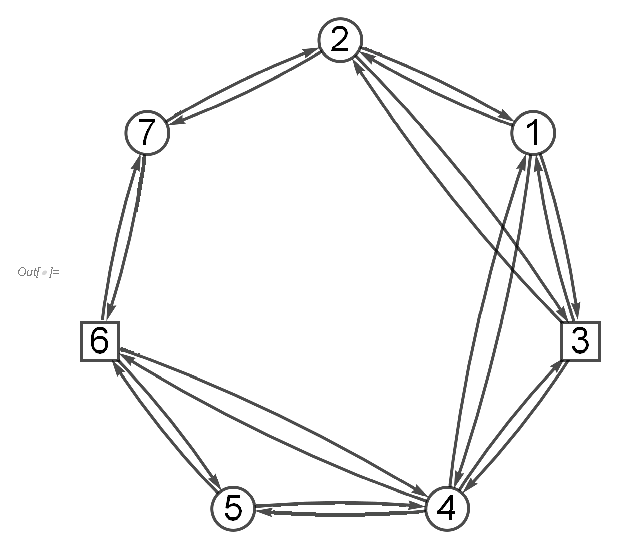
\includegraphics{k1_gr1.eps}

\begin{doublespace}
\noindent\(\pmb{\text{balanceEqs}=\left(\left(\text{Total}\left[x_{\#}\&\text{/@}\text{EdgeList}[g,\_\unicode{f3d5}\#]\right]-\text{Total}\left[x_{\#}\&\text{/@}\text{EdgeList}[g,\#\unicode{f3d5}\_]\right]\right)\right)==\text{MapIndexed}\left[\text{$\#$1}\text{/.}x\to
x_{\text{$\#$2}[[1]]}\&,b\right][[\#]]\&\text{/@}\text{VertexList}[g];}\\
\pmb{\text{balanceEqs}\text{//}\text{forma}}\)
\end{doublespace}

\begin{doublespace}
\noindent\(\begin{array}{l}
 x_{2,7}+x_{6,7}-x_{7,2}-x_{7,6}==0 \\
 x_{1,2}-x_{2,1}-x_{2,3}-x_{2,7}+x_{3,2}+x_{7,2}==0 \\
 x_{4,6}+x_{5,6}-x_{6,4}-x_{6,5}-x_{6,7}+x_{7,6}==x_6 \\
 -x_{1,2}-x_{1,3}-x_{1,4}+x_{2,1}+x_{3,1}+x_{4,1}==0 \\
 x_{1,3}+x_{2,3}-x_{3,1}-x_{3,2}-x_{3,4}+x_{4,3}==x_3 \\
 x_{1,4}+x_{3,4}-x_{4,1}-x_{4,3}-x_{4,5}-x_{4,6}+x_{5,4}+x_{6,4}==0 \\
 x_{4,5}-x_{5,4}-x_{5,6}+x_{6,5}==0 \\
\end{array}\)
\end{doublespace}

\begin{doublespace}
\noindent\(\pmb{M=\{7\};}\\
\pmb{\text{Print}[\text{{``}M = {''}}, M];}\)
\end{doublespace}

\noindent\(\text{M = }\{7\}\)

\begin{doublespace}
\noindent\(\pmb{\text{(*}\text{incL}=\text{DeleteCases}[\text{DeleteDuplicates}[\text{Cases}[\text{IncidenceList}[g,\#],\text{i$\_$}\unicode{f3d5}\text{j$\_$}:\to
\{i,j\}]\text{//}\text{Flatten}],\text{v$\_$}\text{/;}v==\#]\&\text{/@}M\text{*)}}\\
\pmb{\text{incL}=(\text{IncidenceList}[g,\#]\&\text{/@}M)\text{//}\text{Flatten}}\)
\end{doublespace}

\begin{doublespace}
\noindent\(\{7\unicode{f3d5}2,2\unicode{f3d5}7,7\unicode{f3d5}6,6\unicode{f3d5}7\}\)
\end{doublespace}

\begin{doublespace}
\noindent\(\pmb{\text{(*}\text{Do}\left[\text{If}\left[\text{MemberQ}\left[M,j_{[[1]]}\right],b_{[[j[[2]]]]}\text{+=}f_j,b_{[[j[[1]]]]}\text{-=}f_j\right],\{j,\text{incL}\}\right]\text{*)}}\\
\pmb{\bar{b}=\text{Fold}\left[\text{If}\left[\text{MemberQ}\left[M,\text{$\#$2}_{[[1]]}\right],\text{ReplacePart}\left[\#,\text{$\#$2}_{[[2]]}\to
\#_{[[\text{$\#$2}[[2]]]]}+f_{\text{$\#$2}}\right],\text{ReplacePart}\left[\#,\text{$\#$2}_{[[1]]}\to \#_{[[\text{$\#$2}[[1]]]]}-f_{\text{$\#$2}}\right]\right]\&,b,\text{incL}\right];}\\
\pmb{\bar{b}=\text{Delete}\left[\bar{b},\#\right]\&\text{@@}M;}\\
\pmb{\overline{\text{ng}}=\text{VertexDelete}[g,M];}\\
\pmb{\text{GraphPlot}\left[\overline{\text{ng}},\text{EdgeStyle}\to \text{Directive}[\text{Black},\text{Thick}], \text{VertexStyle}\to \text{Directive}[\text{EdgeForm}[\text{Thick}],\text{White}],\text{MultiedgeStyle}\to
.05\right]}\\
\pmb{\bar{b}}\)
\end{doublespace}

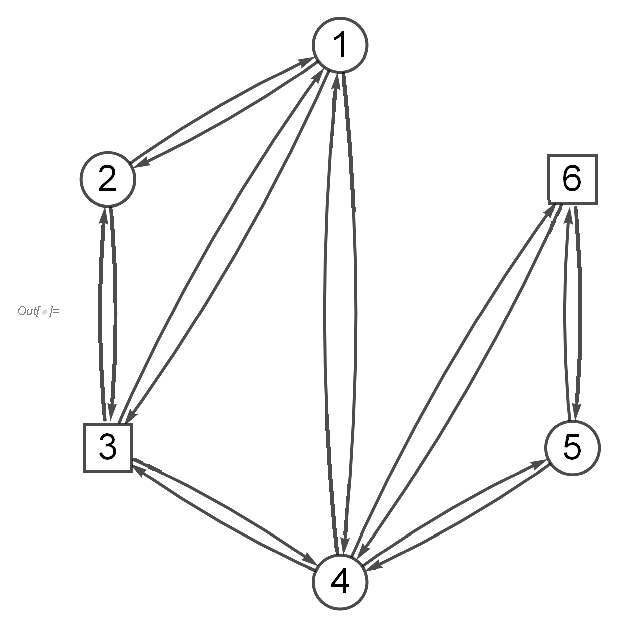
\includegraphics{k1_gr2.eps}

\begin{doublespace}
\noindent\(\left\{0,-f_{2\unicode{f3d5}7}+f_{7\unicode{f3d5}2},x,0,0,x-f_{6\unicode{f3d5}7}+f_{7\unicode{f3d5}6}\right\}\)
\end{doublespace}

\begin{doublespace}
\noindent\(\pmb{\text{CC}[\text{g$\_$},\text{M$\_$}]\text{:=}(\text{DeleteDuplicates}[\text{Cases}[\text{IncidenceList}[g,\#],\text{i$\_$}\unicode{f3d5}\text{j$\_$}\text{/;}j==\#]]\&\text{/@}M)\text{//}\text{Flatten}}\\
\pmb{}\\
\pmb{\text{ii}_{\text{i$\_$}}^+[\text{g$\_$}]\text{:=}\text{Cases}[\text{IncidenceList}[g,i],\text{u$\_$}\unicode{f3d5}\text{v$\_$}\text{/;}u==i:\to
v]}\)
\end{doublespace}

\begin{doublespace}
\noindent\(\pmb{M^+=\text{CC}[g,M]}\)
\end{doublespace}

\begin{doublespace}
\noindent\(\{2\unicode{f3d5}7,6\unicode{f3d5}7\}\)
\end{doublespace}

\begin{doublespace}
\noindent\(\pmb{\overline{\text{b1}}=\text{Fold}\left[\text{Module}\left[\left\{\text{bb}=\text{$\#$1},i=\text{$\#$2}_{[[1]]},k=\text{$\#$2}_{[[2]]}\right\},\left(\text{ReplacePart}\left[\text{bb},
\left(\left(\left(\left\{\#\to \text{bb}_{[[\#]]}+\frac{p_{i\unicode{f3d5}\#}}{p_{i\unicode{f3d5}k}}f_{i\unicode{f3d5}k},i\to \text{bb}_{[[i]]}-\frac{p_{i\unicode{f3d5}\#}}{p_{i\unicode{f3d5}k}}f_{i\unicode{f3d5}k}\right\}\right)\&\right)\text{/@}\text{ii}_i^+\left[\overline{\text{ng}}\right]\right)\text{//}\text{Flatten}\right]\right)\right]\&,\bar{b},M^+\right]}\)
\end{doublespace}

\begin{doublespace}
\noindent\(\left\{\frac{f_{2\unicode{f3d5}7} p_{2\unicode{f3d5}1}}{p_{2\unicode{f3d5}7}},-f_{2\unicode{f3d5}7}+f_{7\unicode{f3d5}2}-\frac{f_{2\unicode{f3d5}7}
p_{2\unicode{f3d5}1}}{p_{2\unicode{f3d5}7}},x+\frac{f_{2\unicode{f3d5}7} p_{2\unicode{f3d5}3}}{p_{2\unicode{f3d5}7}},\frac{f_{6\unicode{f3d5}7} p_{6\unicode{f3d5}4}}{p_{6\unicode{f3d5}7}},\frac{f_{6\unicode{f3d5}7}
p_{6\unicode{f3d5}5}}{p_{6\unicode{f3d5}7}},x-f_{6\unicode{f3d5}7}+f_{7\unicode{f3d5}6}-\frac{f_{6\unicode{f3d5}7} p_{6\unicode{f3d5}5}}{p_{6\unicode{f3d5}7}}\right\}\)
\end{doublespace}

\begin{doublespace}
\noindent\(\pmb{\text{GraphPlot}\left[\text{Fold}\left[\text{HighlightGraph}[\text{$\#$1},\text{u$\_$}\unicode{f3d5}\text{v$\_$}\text{/;}u==\text{$\#$2},
\text{GraphHighlightStyle}\to \text{{``}White{''}}]\&,\overline{\text{ng}},\#_{[[1]]}\&\text{/@}M^+\right],\text{EdgeStyle}\to \text{Directive}[\text{Black},\text{Thick}],
\right.}\\
\pmb{\text{VertexStyle}\to \text{Directive}[\text{EdgeForm}[\text{Thick}],\text{White}],\text{MultiedgeStyle}\to .05]}\)
\end{doublespace}

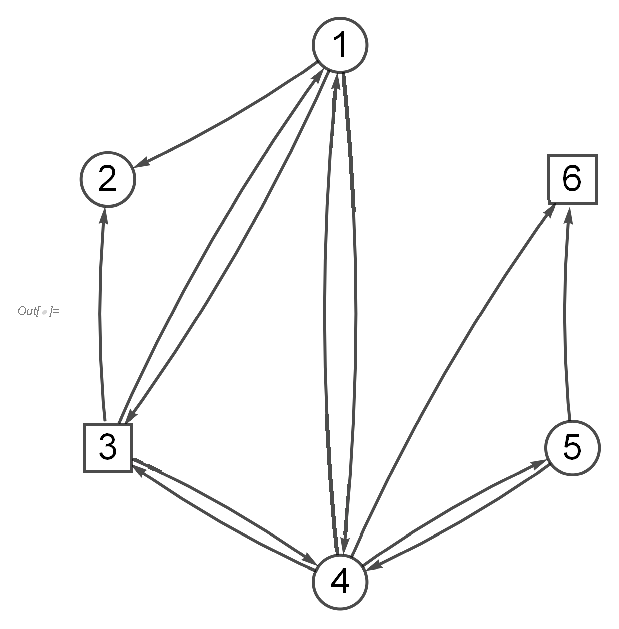
\includegraphics{k1_gr3.eps}

\begin{doublespace}
\noindent\(\pmb{\overline{\text{g1}}=\text{Fold}\left[\text{EdgeDelete}[\text{$\#$1},\text{u$\_$}\unicode{f3d5}\text{v$\_$}\text{/;}u==\text{$\#$2}]\&,\overline{\text{ng}},\#_{[[1]]}\&\text{/@}M^+\right];}\\
\pmb{\text{GraphPlot}\left[\overline{\text{g1}},\text{MultiedgeStyle}\to .05\right]}\)
\end{doublespace}

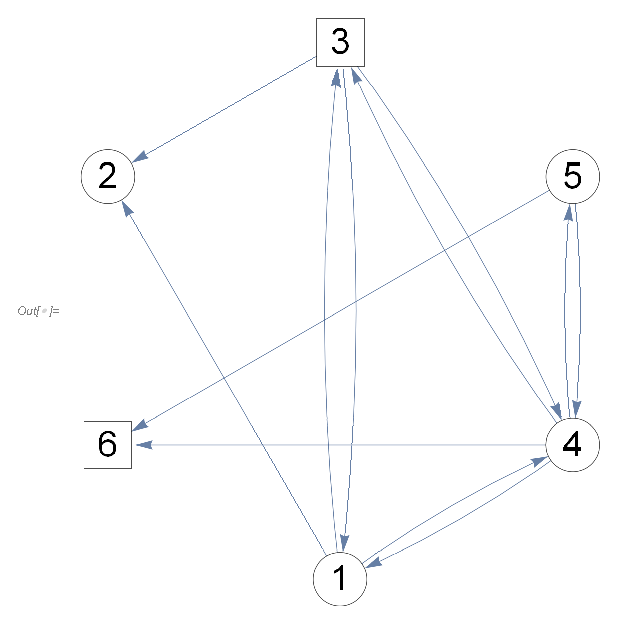
\includegraphics{k1_gr4.eps}

\begin{doublespace}
\noindent\(\pmb{\text{II}_{\text{rem}}=\text{VertexList}\left[\overline{\text{g1}}\right]\sim \text{Complement}\sim \left(M^+[[\text{All},1]]\right)}\)
\end{doublespace}

\begin{doublespace}
\noindent\(\{1,3,4,5\}\)
\end{doublespace}

\begin{doublespace}
\noindent\(\pmb{\lambda =\text{SparseArray}\left[\text{Replace}\left[\left(\text{EdgeList}\left[\overline{\text{g1}}\right]\text{/.}\#\&\text{/@}\text{Flatten}\left[\text{Module}\left[\{i=\#,\text{jf},\text{Icur}\},\left(\text{Icur}=\text{ii}_i^+\left[\overline{\text{g1}}\right];\right.\right.\right.\right.\right.\right.}\\
\pmb{\text{jf}=\text{First}[\text{Icur}];}\\
\pmb{\left.\left.\left.\left.\left.\left.\left(\left\{(i\unicode{f3d5}\text{jf})\to 1,(i\unicode{f3d5}\#)\to - \frac{p_{i\unicode{f3d5}\#}}{p_{i\unicode{f3d5}\text{jf}}}\right\}\right)\&\text{/@}\text{Icur}[[2\text{;;}]]\right)\right]\&\text{/@}\text{II}_{\text{rem}},1\right]\right),\_\unicode{f3d5}\_\to
0,2\right]\right]}\)
\end{doublespace}

\begin{doublespace}
\noindent\(\text{SparseArray}\left[\fbox{$$}\right]\)
\end{doublespace}

\begin{doublespace}
\noindent\(\pmb{\text{Grid}[\lambda ]}\)
\end{doublespace}

\begin{doublespace}
\noindent\(\begin{array}{cccccccccccc}
 1 & 0 & -\frac{p_{1\unicode{f3d5}3}}{p_{1\unicode{f3d5}2}} & 0 & 0 & 0 & 0 & 0 & 0 & 0 & 0 & 0 \\
 1 & 0 & 0 & 0 & -\frac{p_{1\unicode{f3d5}4}}{p_{1\unicode{f3d5}2}} & 0 & 0 & 0 & 0 & 0 & 0 & 0 \\
 0 & 1 & 0 & -\frac{p_{3\unicode{f3d5}1}}{p_{3\unicode{f3d5}2}} & 0 & 0 & 0 & 0 & 0 & 0 & 0 & 0 \\
 0 & 1 & 0 & 0 & 0 & 0 & -\frac{p_{3\unicode{f3d5}4}}{p_{3\unicode{f3d5}2}} & 0 & 0 & 0 & 0 & 0 \\
 0 & 0 & 0 & 0 & 0 & 1 & 0 & -\frac{p_{4\unicode{f3d5}3}}{p_{4\unicode{f3d5}1}} & 0 & 0 & 0 & 0 \\
 0 & 0 & 0 & 0 & 0 & 1 & 0 & 0 & -\frac{p_{4\unicode{f3d5}5}}{p_{4\unicode{f3d5}1}} & 0 & 0 & 0 \\
 0 & 0 & 0 & 0 & 0 & 1 & 0 & 0 & 0 & 0 & 0 & -\frac{p_{4\unicode{f3d5}6}}{p_{4\unicode{f3d5}1}} \\
 0 & 0 & 0 & 0 & 0 & 0 & 0 & 0 & 0 & 1 & -\frac{p_{5\unicode{f3d5}6}}{p_{5\unicode{f3d5}4}} & 0 \\
\end{array}\)
\end{doublespace}

\begin{doublespace}
\noindent\(\pmb{g=\overline{\text{g1}};}\\
\pmb{b=\overline{\text{b1}};}\)
\end{doublespace}

\begin{doublespace}
\noindent\(\pmb{\text{II}^*=\text{Cases}[\text{MapIndexed}[\{\text{$\#$1},\text{$\#$2}\}\&,b],\{\text{el$\_$},\text{i$\_$}\}\text{/;}\text{MemberQ}[\text{el},x]:\to
i]\text{//}\text{Flatten}}\)
\end{doublespace}

\begin{doublespace}
\noindent\(\{3,6\}\)
\end{doublespace}

\begin{doublespace}
\noindent\(\pmb{\text{buildt}=\text{Timing}\left[\{t,g\}=\text{buildTree}\left[g,\text{II}^*\right];\right][[1]]}\\
\pmb{\text{TableForm}[t[[1\text{;;}4]],\text{TableHeadings}\to \{\{\text{{``}pred{''}},\text{{``}dir{''}},\text{{``}depth{''}},\text{d}\},t\text{//}\text{pred}\text{//}\text{Length}\text{//}\text{Range}\}]}\)
\end{doublespace}

\begin{doublespace}
\noindent\(0.015625\)
\end{doublespace}

\begin{doublespace}
\noindent\(\begin{array}{l|l|llllll}
  & 1 & 2 & 3 & 4 & 5 & 6 & 7 \\
\hline
 \text{pred} & 3 & 3 & 7 & 6 & 6 & 7 & 0 \\
\hline
 \text{dir} & 1 & 1 & 1 & -1 & -1 & 1 & 0 \\
 \text{depth} & 2 & 2 & 1 & 2 & 2 & 1 & 0 \\
 \text{d} & 2 & 7 & 1 & 5 & 3 & 4 & 6 \\
\end{array}\)
\end{doublespace}

\begin{doublespace}
\noindent\(\pmb{\text{GraphPlot}\left[\text{HighlightGraph}\left[\text{Fold}\left[\text{HighlightGraph}[\text{$\#$1},\text{Style}[\text{u$\_$}\unicode{f3d5}\text{v$\_$}\text{/;}u==\text{$\#$2},\text{White}]]\&,\overline{\text{ng}},\#_{[[1]]}\&\text{/@}M^+\right],\right.\right.}\\
\pmb{\{\text{Style}[\text{u$\_$}\text{/;}\text{VertexQ}[g,u]\&\&\text{pred}[t][[u]]==7,\text{EdgeForm}[\text{Thick}]],}\\
\pmb{\text{Style}[\text{u$\_$}\unicode{f3d5}\text{v$\_$}\text{/;}(\text{pred}[t][[u]]==v\&\&\text{dir}[t][[u]]==-1)\|(\text{pred}[t][[v]]==u\&\&\text{dir}[t][[v]]==1),\text{Directive}[\text{Black},\text{Thick}]]\},\text{GraphHighlightStyle}\to
\text{None}],}\\
\pmb{\text{MultiedgeStyle}\to .05]}\)
\end{doublespace}

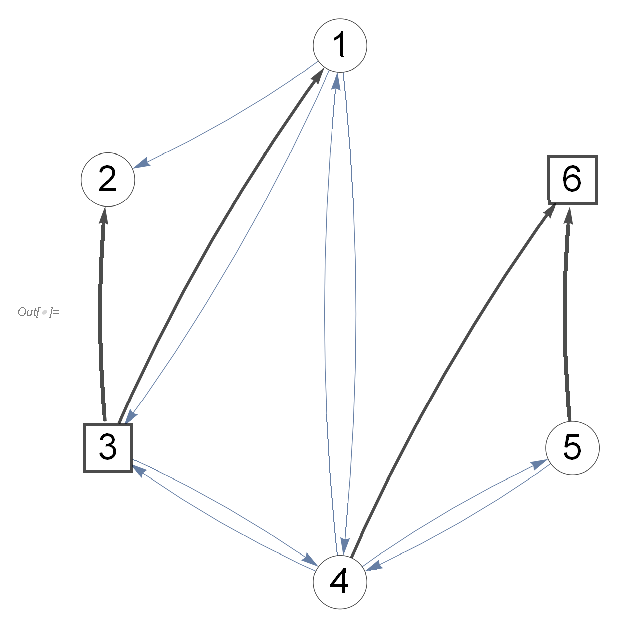
\includegraphics{k1_gr5.eps}

\begin{doublespace}
\noindent\(\pmb{\text{GraphPlot}[}\\
\pmb{\text{HighlightGraph}\left[\overline{\text{g1}},\{\text{Style}[\text{u$\_$}\text{/;}\text{VertexQ}[g,u]\&\&\text{pred}[t][[u]]==7,\text{EdgeForm}[\text{Thick}]],\right.}\\
\pmb{\text{Style}[\text{u$\_$}\unicode{f3d5}\text{v$\_$}\text{/;}(\text{pred}[t][[u]]==v\&\&\text{dir}[t][[u]]==-1)\|(\text{pred}[t][[v]]==u\&\&\text{dir}[t][[v]]==1),\text{Directive}[\text{Black},\text{Thick}]]\},\text{GraphHighlightStyle}\to
\text{None}],}\\
\pmb{\text{MultiedgeStyle}\to .05]}\)
\end{doublespace}

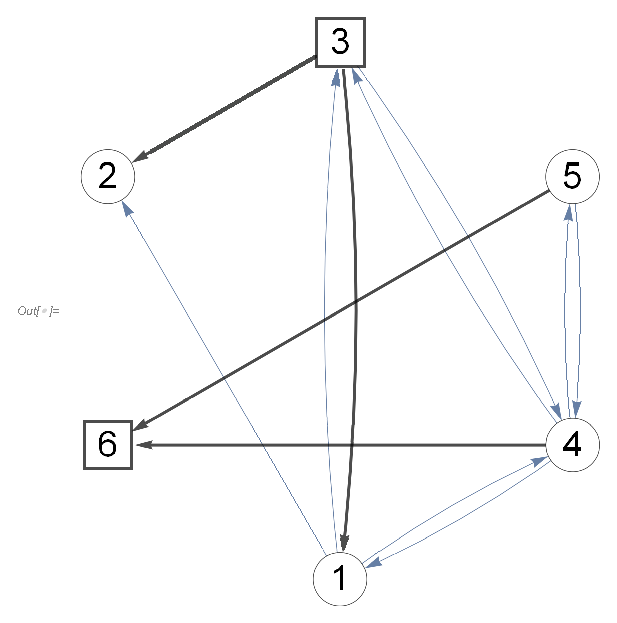
\includegraphics{k1_gr6.eps}

\begin{doublespace}
\noindent\(\pmb{\text{VertexDelete}[t[[7]],7]\text{(*$\unicode{043f}\unicode{043e}\unicode{043c}\unicode{0435}\unicode{0442}\unicode{0438}\unicode{0442}\unicode{044c}$
$\unicode{043d}\unicode{0430}$ $\unicode{0433}\unicode{0440}\unicode{0430}\unicode{0444}\unicode{0435}$*)}}\)
\end{doublespace}

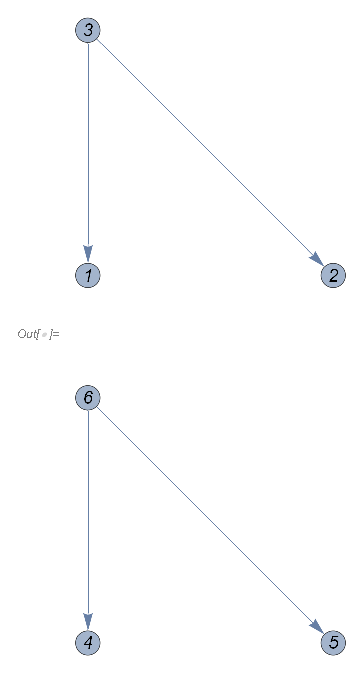
\includegraphics{k1_gr7.eps}

\begin{doublespace}
\noindent\(\pmb{\text{GraphPlot}[g,\text{MultiedgeStyle}\to .05]}\)
\end{doublespace}

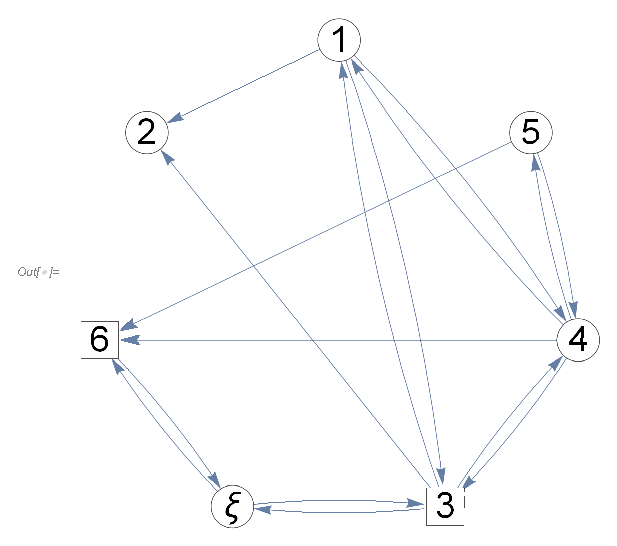
\includegraphics{k1_gr8.eps}

\begin{doublespace}
\noindent\(\pmb{\text{AppendTo}[b,-\text{Total}[b]];}\\
\pmb{b=\text{Simplify}[b\text{/.}x\to 0]}\)
\end{doublespace}

\begin{doublespace}
\noindent\(\left\{\frac{f_{2\unicode{f3d5}7} p_{2\unicode{f3d5}1}}{p_{2\unicode{f3d5}7}},f_{7\unicode{f3d5}2}+f_{2\unicode{f3d5}7} \left(-1-\frac{p_{2\unicode{f3d5}1}}{p_{2\unicode{f3d5}7}}\right),\frac{f_{2\unicode{f3d5}7}
p_{2\unicode{f3d5}3}}{p_{2\unicode{f3d5}7}},\frac{f_{6\unicode{f3d5}7} p_{6\unicode{f3d5}4}}{p_{6\unicode{f3d5}7}},\frac{f_{6\unicode{f3d5}7} p_{6\unicode{f3d5}5}}{p_{6\unicode{f3d5}7}},f_{7\unicode{f3d5}6}+f_{6\unicode{f3d5}7}
\left(-1-\frac{p_{6\unicode{f3d5}5}}{p_{6\unicode{f3d5}7}}\right),-f_{7\unicode{f3d5}2}-f_{7\unicode{f3d5}6}+f_{2\unicode{f3d5}7} \left(1-\frac{p_{2\unicode{f3d5}3}}{p_{2\unicode{f3d5}7}}\right)+f_{6\unicode{f3d5}7}
\left(1-\frac{p_{6\unicode{f3d5}4}}{p_{6\unicode{f3d5}7}}\right)\right\}\)
\end{doublespace}

\begin{doublespace}
\noindent\(\pmb{\text{balanceEqs}=\left(\left(\text{Total}\left[x_{\#}\&\text{/@}\text{EdgeList}[g,\_\unicode{f3d5}\#]\right]-\text{Total}\left[x_{\#}\&\text{/@}\text{EdgeList}[g,\#\unicode{f3d5}\_]\right]\right)\text{/.}
7\to \xi \right)==b[[\#]]\&\text{/@}\text{VertexList}[g];}\\
\pmb{\text{balanceEqs}\text{//}\text{forma}}\)
\end{doublespace}

\begin{doublespace}
\noindent\(\begin{array}{l}
 x_{1,2}+x_{3,2}==f_{7,2}+f_{2,7} \left(-1-\frac{p_{2,1}}{p_{2,7}}\right) \\
 x_{4,6}+x_{5,6}-x_{6,\xi }+x_{\xi ,6}==f_{7,6}+f_{6,7} \left(-1-\frac{p_{6,5}}{p_{6,7}}\right) \\
 -x_{1,2}-x_{1,3}-x_{1,4}+x_{3,1}+x_{4,1}==\frac{f_{2,7} p_{2,1}}{p_{2,7}} \\
 x_{1,3}-x_{3,1}-x_{3,2}-x_{3,4}-x_{3,\xi }+x_{4,3}+x_{\xi ,3}==\frac{f_{2,7} p_{2,3}}{p_{2,7}} \\
 x_{1,4}+x_{3,4}-x_{4,1}-x_{4,3}-x_{4,5}-x_{4,6}+x_{5,4}==\frac{f_{6,7} p_{6,4}}{p_{6,7}} \\
 x_{4,5}-x_{5,4}-x_{5,6}==\frac{f_{6,7} p_{6,5}}{p_{6,7}} \\
 x_{3,\xi }+x_{6,\xi }-x_{\xi ,3}-x_{\xi ,6}==-f_{7,2}-f_{7,6}+f_{2,7} \left(1-\frac{p_{2,3}}{p_{2,7}}\right)+f_{6,7} \left(1-\frac{p_{6,4}}{p_{6,7}}\right)
\\
\end{array}\)
\end{doublespace}

\begin{doublespace}
\noindent\(\pmb{\text{ps}=\text{partSolve}\left[g,-b,t,\tilde{x}\right];}\\
\pmb{\text{ps}\text{//}\text{forma}}\)
\end{doublespace}

\noindent\(7\)

\begin{doublespace}
\noindent\(\begin{array}{l}
 \tilde{x}_{1,2}\to 0 \\
 \tilde{x}_{1,3}\to 0 \\
 \tilde{x}_{1,4}\to 0 \\
 \tilde{x}_{3,1}\to \frac{f_{2,7} p_{2,1}}{p_{2,7}} \\
 \tilde{x}_{3,2}\to f_{7,2}+f_{2,7} \left(-1-\frac{p_{2,1}}{p_{2,7}}\right) \\
 \tilde{x}_{3,4}\to 0 \\
 \tilde{x}_{3,7}\to 0 \\
 \tilde{x}_{4,1}\to 0 \\
 \tilde{x}_{4,3}\to 0 \\
 \tilde{x}_{4,5}\to 0 \\
 \tilde{x}_{4,6}\to -\frac{f_{6,7} p_{6,4}}{p_{6,7}} \\
 \tilde{x}_{5,4}\to 0 \\
 \tilde{x}_{5,6}\to -\frac{f_{6,7} p_{6,5}}{p_{6,7}} \\
 \tilde{x}_{6,7}\to 0 \\
 \tilde{x}_{7,3}\to f_{7,2}+f_{2,7} \left(-1-\frac{p_{2,1}}{p_{2,7}}\right)+\frac{f_{2,7} p_{2,1}}{p_{2,7}}+\frac{f_{2,7} p_{2,3}}{p_{2,7}} \\
 \tilde{x}_{7,6}\to f_{7,6}+f_{6,7} \left(-1-\frac{p_{6,5}}{p_{6,7}}\right)+\frac{f_{6,7} p_{6,4}}{p_{6,7}}+\frac{f_{6,7} p_{6,5}}{p_{6,7}} \\
\end{array}\)
\end{doublespace}

\begin{doublespace}
\noindent\(\pmb{\text{Simplify}\left[\left(\text{balanceEqs}\text{/.}\left\{x\to \tilde{x},\xi \to 7\right\}\right)\text{/.}\text{ps}\right]}\)
\end{doublespace}

\begin{doublespace}
\noindent\(\{\text{True},\text{True},\text{True},\text{True},\text{True},\text{True},\text{True}\}\)
\end{doublespace}

\begin{doublespace}
\noindent\(\pmb{\text{matrt}=\text{Timing}[\text{$\delta $Matr}=\text{$\delta $1}[g,t]];}\\
\pmb{\text{roott}=\text{VertexCount}[g];}\\
\pmb{\text{TableForm}\left[\text{$\delta $Matr},\text{TableHeadings}\to \left\{\text{uNb}[g,t],\delta _{\begin{cases}
 \#_{[[2]]} & \#_{[[1]]}== \text{roott} \\
 \#_{[[1]]} & \#[[2]]==\text{roott} \\
 \# & \text{True}
\end{cases}
}\&\text{/@}\text{EdgeList}[g]\right\}\right]\text{//}\text{forma}}\)
\end{doublespace}

\begin{doublespace}
\noindent\(\begin{array}{l|llllllllllllllll}
  & \delta _{1,2} & \delta _{3,2} & \delta _{1,3} & \delta _{3,1} & \delta _{1,4} & \delta _{4,1} & \delta _{3,4} & \delta _{4,3} & \delta _{4,5}
& \delta _{5,4} & \delta _{5,6} & \delta _{4,6} & \delta _3 & \delta _6 & \delta _3 & \delta _6 \\
\hline
 1\unicode{f3d5}2 & 1 & -1 & 0 & 1 & 0 & 0 & 0 & 0 & 0 & 0 & 0 & 0 & 0 & 0 & 0 & 0 \\
 1\unicode{f3d5}3 & 0 & 0 & 1 & 1 & 0 & 0 & 0 & 0 & 0 & 0 & 0 & 0 & 0 & 0 & 0 & 0 \\
 1\unicode{f3d5}4 & 0 & 0 & 0 & 1 & 1 & 0 & 0 & 0 & 0 & 0 & 0 & 1 & 1 & -1 & 0 & 0 \\
 4\unicode{f3d5}1 & 0 & 0 & 0 & -1 & 0 & 1 & 0 & 0 & 0 & 0 & 0 & -1 & -1 & 1 & 0 & 0 \\
 3\unicode{f3d5}4 & 0 & 0 & 0 & 0 & 0 & 0 & 1 & 0 & 0 & 0 & 0 & 1 & 1 & -1 & 0 & 0 \\
 4\unicode{f3d5}3 & 0 & 0 & 0 & 0 & 0 & 0 & 0 & 1 & 0 & 0 & 0 & -1 & -1 & 1 & 0 & 0 \\
 4\unicode{f3d5}5 & 0 & 0 & 0 & 0 & 0 & 0 & 0 & 0 & 1 & 0 & 1 & -1 & 0 & 0 & 0 & 0 \\
 5\unicode{f3d5}4 & 0 & 0 & 0 & 0 & 0 & 0 & 0 & 0 & 0 & 1 & -1 & 1 & 0 & 0 & 0 & 0 \\
 3\unicode{f3d5}7 & 0 & 0 & 0 & 0 & 0 & 0 & 0 & 0 & 0 & 0 & 0 & 0 & 1 & 0 & 1 & 0 \\
 6\unicode{f3d5}7 & 0 & 0 & 0 & 0 & 0 & 0 & 0 & 0 & 0 & 0 & 0 & 0 & 0 & 1 & 0 & 1 \\
\end{array}\)
\end{doublespace}

\begin{doublespace}
\noindent\(\pmb{\lambda =\text{SparseArray}[\lambda ,\{\text{Length}[\lambda ],\text{Length}[\lambda [[1]]]+4\}];}\\
\pmb{\text{(*}\lambda =\lambda [[\text{;;}-2]]\text{*)}}\)
\end{doublespace}

\begin{doublespace}
\noindent\(\pmb{\text{dopEq}=\#==0\&\text{/@}\text{Flatten}\left[\lambda .\left\{x_{\#}\&\text{/@}\text{EdgeList}[g]\right\}{}^{\mathsf{T}}\right];}\\
\pmb{\text{dopEq}\text{//}\text{forma}}\)
\end{doublespace}

\begin{doublespace}
\noindent\(\begin{array}{l}
 x_{1,2}-\frac{p_{1,3} x_{1,3}}{p_{1,2}}==0 \\
 x_{1,2}-\frac{p_{1,4} x_{1,4}}{p_{1,2}}==0 \\
 -\frac{p_{3,1} x_{3,1}}{p_{3,2}}+x_{3,2}==0 \\
 x_{3,2}-\frac{p_{3,4} x_{3,4}}{p_{3,2}}==0 \\
 x_{4,1}-\frac{p_{4,3} x_{4,3}}{p_{4,1}}==0 \\
 x_{4,1}-\frac{p_{4,5} x_{4,5}}{p_{4,1}}==0 \\
 x_{4,1}-\frac{p_{4,6} x_{4,6}}{p_{4,1}}==0 \\
 x_{5,4}-\frac{p_{5,6} x_{5,6}}{p_{5,4}}==0 \\
\end{array}\)
\end{doublespace}

\begin{doublespace}
\noindent\(\pmb{\Lambda =\lambda .(\text{$\delta $Matr})^{\mathsf{T}};}\\
\pmb{\text{{``}cicle det's:{''}}}\\
\pmb{\Lambda \text{//}\text{forma}}\)
\end{doublespace}

\begin{doublespace}
\noindent\(\text{cicle det's:}\)
\end{doublespace}

\begin{doublespace}
\noindent\(\begin{array}{llllllllll}
 1 & -\frac{p_{1\unicode{f3d5}3}}{p_{1\unicode{f3d5}2}} & 0 & 0 & 0 & 0 & 0 & 0 & 0 & 0 \\
 1 & 0 & -\frac{p_{1\unicode{f3d5}4}}{p_{1\unicode{f3d5}2}} & 0 & 0 & 0 & 0 & 0 & 0 & 0 \\
 -1-\frac{p_{3\unicode{f3d5}1}}{p_{3\unicode{f3d5}2}} & -\frac{p_{3\unicode{f3d5}1}}{p_{3\unicode{f3d5}2}} & -\frac{p_{3\unicode{f3d5}1}}{p_{3\unicode{f3d5}2}}
& \frac{p_{3\unicode{f3d5}1}}{p_{3\unicode{f3d5}2}} & 0 & 0 & 0 & 0 & 0 & 0 \\
 -1 & 0 & 0 & 0 & -\frac{p_{3\unicode{f3d5}4}}{p_{3\unicode{f3d5}2}} & 0 & 0 & 0 & 0 & 0 \\
 0 & 0 & 0 & 1 & 0 & -\frac{p_{4\unicode{f3d5}3}}{p_{4\unicode{f3d5}1}} & 0 & 0 & 0 & 0 \\
 0 & 0 & 0 & 1 & 0 & 0 & -\frac{p_{4\unicode{f3d5}5}}{p_{4\unicode{f3d5}1}} & 0 & 0 & 0 \\
 0 & 0 & -\frac{p_{4\unicode{f3d5}6}}{p_{4\unicode{f3d5}1}} & 1+\frac{p_{4\unicode{f3d5}6}}{p_{4\unicode{f3d5}1}} & -\frac{p_{4\unicode{f3d5}6}}{p_{4\unicode{f3d5}1}}
& \frac{p_{4\unicode{f3d5}6}}{p_{4\unicode{f3d5}1}} & \frac{p_{4\unicode{f3d5}6}}{p_{4\unicode{f3d5}1}} & -\frac{p_{4\unicode{f3d5}6}}{p_{4\unicode{f3d5}1}}
& 0 & 0 \\
 0 & 0 & 0 & 0 & 0 & 0 & -\frac{p_{5\unicode{f3d5}6}}{p_{5\unicode{f3d5}4}} & 1+\frac{p_{5\unicode{f3d5}6}}{p_{5\unicode{f3d5}4}} & 0 & 0 \\
\end{array}\)
\end{doublespace}

\begin{doublespace}
\noindent\(\pmb{\texttt{"}U_c\text{=$\texttt{"}$}}\\
\pmb{U_c=\text{Range}[8]}\\
\pmb{\texttt{"}U_{\text{nc}}\text{=$\texttt{"}$}}\\
\pmb{U_{\text{nc}}=\{9,10\}}\)
\end{doublespace}

\begin{doublespace}
\noindent\(U_c=\)
\end{doublespace}

\begin{doublespace}
\noindent\(\{1,2,3,4,5,6,7,8\}\)
\end{doublespace}

\begin{doublespace}
\noindent\(U_{\text{nc}}=\)
\end{doublespace}

\begin{doublespace}
\noindent\(\{9,10\}\)
\end{doublespace}

\begin{doublespace}
\noindent\(\pmb{\text{$\Lambda $c}=\Lambda \left[\left[\text{All},U_c\right]\right];}\\
\pmb{\text{$\Lambda $nc}=\Lambda \left[\left[\text{All},U_{\text{nc}}\right]\right];}\\
\pmb{\texttt{"}\Lambda _c\text{=$\texttt{"}$}}\\
\pmb{\text{$\Lambda $c}\text{//}\text{MatrixForm}}\)
\end{doublespace}

\begin{doublespace}
\noindent\(\Lambda _c=\)
\end{doublespace}

\begin{doublespace}
\noindent\(\left(
\begin{array}{cccccccc}
 1 & -\frac{p_{1\unicode{f3d5}3}}{p_{1\unicode{f3d5}2}} & 0 & 0 & 0 & 0 & 0 & 0 \\
 1 & 0 & -\frac{p_{1\unicode{f3d5}4}}{p_{1\unicode{f3d5}2}} & 0 & 0 & 0 & 0 & 0 \\
 -1-\frac{p_{3\unicode{f3d5}1}}{p_{3\unicode{f3d5}2}} & -\frac{p_{3\unicode{f3d5}1}}{p_{3\unicode{f3d5}2}} & -\frac{p_{3\unicode{f3d5}1}}{p_{3\unicode{f3d5}2}}
& \frac{p_{3\unicode{f3d5}1}}{p_{3\unicode{f3d5}2}} & 0 & 0 & 0 & 0 \\
 -1 & 0 & 0 & 0 & -\frac{p_{3\unicode{f3d5}4}}{p_{3\unicode{f3d5}2}} & 0 & 0 & 0 \\
 0 & 0 & 0 & 1 & 0 & -\frac{p_{4\unicode{f3d5}3}}{p_{4\unicode{f3d5}1}} & 0 & 0 \\
 0 & 0 & 0 & 1 & 0 & 0 & -\frac{p_{4\unicode{f3d5}5}}{p_{4\unicode{f3d5}1}} & 0 \\
 0 & 0 & -\frac{p_{4\unicode{f3d5}6}}{p_{4\unicode{f3d5}1}} & 1+\frac{p_{4\unicode{f3d5}6}}{p_{4\unicode{f3d5}1}} & -\frac{p_{4\unicode{f3d5}6}}{p_{4\unicode{f3d5}1}}
& \frac{p_{4\unicode{f3d5}6}}{p_{4\unicode{f3d5}1}} & \frac{p_{4\unicode{f3d5}6}}{p_{4\unicode{f3d5}1}} & -\frac{p_{4\unicode{f3d5}6}}{p_{4\unicode{f3d5}1}}
\\
 0 & 0 & 0 & 0 & 0 & 0 & -\frac{p_{5\unicode{f3d5}6}}{p_{5\unicode{f3d5}4}} & 1+\frac{p_{5\unicode{f3d5}6}}{p_{5\unicode{f3d5}4}} \\
\end{array}
\right)\)
\end{doublespace}

\begin{doublespace}
\noindent\(\pmb{\text{$\texttt{"}$det(}\Lambda _c\text{)=$\texttt{"}$}}\\
\pmb{\text{Simplify}[\det =\text{Det}[\text{$\Lambda $c}]]\text{//}\text{forma}}\)
\end{doublespace}

\begin{doublespace}
\noindent\(\text{det(}\Lambda _c\text{)=}\)
\end{doublespace}

\begin{doublespace}
\noindent\(-\frac{1}{p_{1,2}^2 p_{3,2}^2 p_{4,1}^3 p_{5,4}}\left(p_{1,2} p_{3,1} p_{3,4} \left(p_{1,3} p_{4,1} \left(p_{4,5} p_{4,6} \left(p_{5,4}+p_{5,6}\right)+p_{4,3}
\left(p_{4,6} p_{5,4}+p_{4,5} \left(p_{5,4}+p_{5,6}\right)\right)\right)+p_{1,4} \left(p_{4,3} p_{4,5} p_{4,6} \left(p_{5,4}+p_{5,6}\right)+p_{4,1}
\left(p_{4,5} p_{4,6} \left(p_{5,4}+p_{5,6}\right)+p_{4,3} \left(p_{4,6} p_{5,4}+p_{4,5} \left(p_{5,4}+p_{5,6}\right)\right)\right)\right)\right)+p_{1,3}
p_{1,4} \left(p_{3,2} p_{3,4} \left(p_{4,3} p_{4,5} p_{4,6} \left(p_{5,4}+p_{5,6}\right)+p_{4,1} \left(p_{4,5} p_{4,6} \left(p_{5,4}+p_{5,6}\right)+p_{4,3}
\left(p_{4,6} p_{5,4}+p_{4,5} \left(p_{5,4}+p_{5,6}\right)\right)\right)\right)+p_{3,1} \left(p_{3,2} p_{4,3} p_{4,5} p_{4,6} \left(p_{5,4}+p_{5,6}\right)+p_{3,4}
\left(p_{4,3} p_{4,5} p_{4,6} \left(p_{5,4}+p_{5,6}\right)+p_{4,1} \left(p_{4,5} p_{4,6} \left(p_{5,4}+p_{5,6}\right)+p_{4,3} \left(p_{4,6} p_{5,4}+p_{4,5}
\left(p_{5,4}+p_{5,6}\right)\right)\right)\right)\right)\right)\right)\)
\end{doublespace}

\begin{doublespace}
\noindent\(\pmb{\texttt{"}U_T\text{=$\texttt{"}$}}\\
\pmb{\text{utind}=\text{Cases}[t[[6]],\xi \_\text{/;}\xi \neq 0];}\\
\pmb{U_T=\text{EdgeList}[g][[\text{utind}]]}\)
\end{doublespace}

\begin{doublespace}
\noindent\(U_T=\)
\end{doublespace}

\begin{doublespace}
\noindent\(\{3\unicode{f3d5}1,3\unicode{f3d5}2,7\unicode{f3d5}3,4\unicode{f3d5}6,5\unicode{f3d5}6,7\unicode{f3d5}6\}\)
\end{doublespace}

\begin{doublespace}
\noindent\(\pmb{\texttt{"}U_{\text{Nb}}\text{=$\texttt{"}$}}\\
\pmb{U_{\text{Nb}}=\text{uNb}[g,t]}\)
\end{doublespace}

\begin{doublespace}
\noindent\(U_{\text{Nb}}=\)
\end{doublespace}

\begin{doublespace}
\noindent\(\{1\unicode{f3d5}2,1\unicode{f3d5}3,1\unicode{f3d5}4,4\unicode{f3d5}1,3\unicode{f3d5}4,4\unicode{f3d5}3,4\unicode{f3d5}5,5\unicode{f3d5}4,3\unicode{f3d5}7,6\unicode{f3d5}7\}\)
\end{doublespace}

\begin{doublespace}
\noindent\(\pmb{A=-\lambda .\left\{\tilde{x}_{\#}\&\text{/@}\text{EdgeList}[g]\right\}{}^{\mathsf{T}}\text{/.}\text{ps};}\\
\pmb{\text{{``}A={''}}}\\
\pmb{A\text{//}\text{MatrixForm}}\)
\end{doublespace}

\begin{doublespace}
\noindent\(\text{A=}\)
\end{doublespace}

\begin{doublespace}
\noindent\(\left(
\begin{array}{c}
 0 \\
 0 \\
 -f_{7\unicode{f3d5}2}-f_{2\unicode{f3d5}7} \left(-1-\frac{p_{2\unicode{f3d5}1}}{p_{2\unicode{f3d5}7}}\right)+\frac{f_{2\unicode{f3d5}7} p_{2\unicode{f3d5}1}
p_{3\unicode{f3d5}1}}{p_{2\unicode{f3d5}7} p_{3\unicode{f3d5}2}} \\
 -f_{7\unicode{f3d5}2}-f_{2\unicode{f3d5}7} \left(-1-\frac{p_{2\unicode{f3d5}1}}{p_{2\unicode{f3d5}7}}\right) \\
 0 \\
 0 \\
 -\frac{f_{6\unicode{f3d5}7} p_{4\unicode{f3d5}6} p_{6\unicode{f3d5}4}}{p_{4\unicode{f3d5}1} p_{6\unicode{f3d5}7}} \\
 -\frac{f_{6\unicode{f3d5}7} p_{5\unicode{f3d5}6} p_{6\unicode{f3d5}5}}{p_{5\unicode{f3d5}4} p_{6\unicode{f3d5}7}} \\
\end{array}
\right)\)
\end{doublespace}

\begin{doublespace}
\noindent\(\pmb{\beta =A-\text{$\Lambda $nc}.\left\{x_{\#}\&\text{/@}U_{\text{Nb}}\left[\left[U_{\text{nc}}\right]\right]\right\}{}^{\mathsf{T}};}\\
\pmb{\text{{``}$\beta $={''}}}\\
\pmb{\beta \text{//}\text{forma}}\)
\end{doublespace}

\begin{doublespace}
\noindent\(\text{$\beta $=}\)
\end{doublespace}

\begin{doublespace}
\noindent\(\begin{array}{l}
 0 \\
 0 \\
 -f_{7,2}-f_{2,7} \left(-1-\frac{p_{2,1}}{p_{2,7}}\right)+\frac{f_{2,7} p_{2,1} p_{3,1}}{p_{2,7} p_{3,2}} \\
 -f_{7,2}-f_{2,7} \left(-1-\frac{p_{2,1}}{p_{2,7}}\right) \\
 0 \\
 0 \\
 -\frac{f_{6,7} p_{4,6} p_{6,4}}{p_{4,1} p_{6,7}} \\
 -\frac{f_{6,7} p_{5,6} p_{6,5}}{p_{5,4} p_{6,7}} \\
\end{array}\)
\end{doublespace}

\begin{doublespace}
\noindent\(\pmb{\text{$\texttt{"}\unicode{0440}\unicode{0435}\unicode{0448}\unicode{0430}\unicode{0435}\unicode{043c}$ $\unicode{0443}\unicode{0440}\unicode{0430}\unicode{0432}\unicode{043d}\unicode{0435}\unicode{043d}\unicode{0438}\unicode{0435}$
}\Lambda _cx_c\text{=$\beta $:$\texttt{"}$}}\\
\pmb{\text{xc}=\text{LinearSolve}[\text{$\Lambda $c},\beta ]}\)
\end{doublespace}

\begin{doublespace}
\noindent\(\text{$\unicode{0440}\unicode{0435}\unicode{0448}\unicode{0430}\unicode{0435}\unicode{043c}$ $\unicode{0443}\unicode{0440}\unicode{0430}\unicode{0432}\unicode{043d}\unicode{0435}\unicode{043d}\unicode{0438}\unicode{0435}$
}\Lambda _cx_c\text{=$\beta $:}\)
\end{doublespace}

\begin{doublespace}
\noindent\(\fbox{$
\begin{array}{l}
  \\
 
\begin{array}{c|cccc}
  & \fbox{$\text{}$} & \fbox{$\text{}$} & \fbox{$\text{}$} & \fbox{$\text{}$} \\
\end{array}
 \\
\end{array}
$}\)
\end{doublespace}

\begin{doublespace}
\noindent\(\pmb{\text{xcp}=\text{MapThread}\left[x_{\text{$\#$1}}\to \text{$\#$2}\&,\left\{U_{\text{Nb}}\left[\left[U_c\right]\right],\text{Flatten}[\text{xc}]\right\}\right];}\\
\pmb{\text{xcp}\text{//}\text{TableForm}}\)
\end{doublespace}

\begin{doublespace}
\noindent\(\fbox{$
\begin{array}{l}
  \\
 
\begin{array}{c|cccc}
  & \fbox{$\text{}$} & \fbox{$\text{}$} & \fbox{$\text{}$} & \fbox{$\text{}$} \\
\end{array}
 \\
\end{array}
$}\)
\end{doublespace}

\begin{doublespace}
\noindent\(\pmb{s=\text{solveAll}[g,t];}\\
\pmb{s\text{//}\text{TableForm}}\)
\end{doublespace}

\begin{doublespace}
\noindent\(\begin{array}{l}
 x_{3\unicode{f3d5}2}\to f_{7\unicode{f3d5}2}+f_{2\unicode{f3d5}7} \left(-1-\frac{p_{2\unicode{f3d5}1}}{p_{2\unicode{f3d5}7}}\right)-x_{1\unicode{f3d5}2}
\\
 x_{3\unicode{f3d5}1}\to \frac{f_{2\unicode{f3d5}7} p_{2\unicode{f3d5}1}}{p_{2\unicode{f3d5}7}}+x_{1\unicode{f3d5}2}+x_{1\unicode{f3d5}3}+x_{1\unicode{f3d5}4}-x_{4\unicode{f3d5}1}
\\
 x_{5\unicode{f3d5}6}\to -\frac{f_{6\unicode{f3d5}7} p_{6\unicode{f3d5}5}}{p_{6\unicode{f3d5}7}}+x_{4\unicode{f3d5}5}-x_{5\unicode{f3d5}4} \\
 x_{4\unicode{f3d5}6}\to -\frac{f_{6\unicode{f3d5}7} p_{6\unicode{f3d5}4}}{p_{6\unicode{f3d5}7}}+x_{1\unicode{f3d5}4}+x_{3\unicode{f3d5}4}-x_{4\unicode{f3d5}1}-x_{4\unicode{f3d5}3}-x_{4\unicode{f3d5}5}+x_{5\unicode{f3d5}4}
\\
 x_{7\unicode{f3d5}3}\to f_{7\unicode{f3d5}2}+f_{2\unicode{f3d5}7} \left(-1-\frac{p_{2\unicode{f3d5}1}}{p_{2\unicode{f3d5}7}}\right)+\frac{f_{2\unicode{f3d5}7}
p_{2\unicode{f3d5}1}}{p_{2\unicode{f3d5}7}}+\frac{f_{2\unicode{f3d5}7} p_{2\unicode{f3d5}3}}{p_{2\unicode{f3d5}7}}+x_{1\unicode{f3d5}4}+x_{3\unicode{f3d5}4}+x_{3\unicode{f3d5}7}-x_{4\unicode{f3d5}1}-x_{4\unicode{f3d5}3}
\\
 x_{7\unicode{f3d5}6}\to f_{7\unicode{f3d5}6}+f_{6\unicode{f3d5}7} \left(-1-\frac{p_{6\unicode{f3d5}5}}{p_{6\unicode{f3d5}7}}\right)+\frac{f_{6\unicode{f3d5}7}
p_{6\unicode{f3d5}4}}{p_{6\unicode{f3d5}7}}+\frac{f_{6\unicode{f3d5}7} p_{6\unicode{f3d5}5}}{p_{6\unicode{f3d5}7}}-x_{1\unicode{f3d5}4}-x_{3\unicode{f3d5}4}+x_{4\unicode{f3d5}1}+x_{4\unicode{f3d5}3}+x_{6\unicode{f3d5}7}
\\
\end{array}\)
\end{doublespace}

\begin{doublespace}
\noindent\(\pmb{\text{{``}$\unicode{043e}\unicode{0431}\unicode{0449}\unicode{0435}\unicode{0435}$ $\unicode{0440}\unicode{0435}\unicode{0448}\unicode{0435}\unicode{043d}\unicode{0438}\unicode{0435}$:{''}}}\\
\pmb{\text{xsol}=(s\sim \text{Join}\sim \text{xcp});}\\
\pmb{\text{xsol}\text{/.}\left\{\xi \__{\text{u$\_$}\unicode{f3d5}\text{v$\_$}}\to \xi _{u,v}\right\}\text{//}\text{Simplify}\text{//}\text{TableForm}}\)
\end{doublespace}

\begin{doublespace}
\noindent\(\text{$\unicode{043e}\unicode{0431}\unicode{0449}\unicode{0435}\unicode{0435}$ $\unicode{0440}\unicode{0435}\unicode{0448}\unicode{0435}\unicode{043d}\unicode{0438}\unicode{0435}$:}\)
\end{doublespace}

\begin{doublespace}
\noindent\(\begin{array}{l}
 x_{3,2}\to f_{7,2}+f_{2,7} \left(-1-\frac{p_{2,1}}{p_{2,7}}\right)-x_{1,2} \\
 x_{3,1}\to \frac{f_{2,7} p_{2,1}}{p_{2,7}}+x_{1,2}+x_{1,3}+x_{1,4}-x_{4,1} \\
 x_{5,6}\to -\frac{f_{6,7} p_{6,5}}{p_{6,7}}+x_{4,5}-x_{5,4} \\
 x_{4,6}\to -\frac{f_{6,7} p_{6,4}}{p_{6,7}}+x_{1,4}+x_{3,4}-x_{4,1}-x_{4,3}-x_{4,5}+x_{5,4} \\
 x_{7,3}\to f_{7,2}+f_{2,7} \left(-1+\frac{p_{2,3}}{p_{2,7}}\right)+x_{1,4}+x_{3,4}+x_{3,7}-x_{4,1}-x_{4,3} \\
 x_{7,6}\to f_{7,6}+f_{6,7} \left(-1+\frac{p_{6,4}}{p_{6,7}}\right)-x_{1,4}-x_{3,4}+x_{4,1}+x_{4,3}+x_{6,7} \\
 x_{1,2}\to -\frac{p_{1,3} p_{1,4} \left(f_{6,7} p_{2,7} p_{3,1} p_{3,4} p_{4,3} p_{4,5} p_{4,6} \left(p_{5,4} p_{6,4}+p_{5,6} \left(p_{6,4}+p_{6,5}\right)\right)+\left(-f_{7,2}
p_{2,7} p_{3,2} \left(p_{3,1} p_{4,3} p_{4,5} p_{4,6} \left(p_{5,4}+p_{5,6}\right)+p_{3,4} \left(p_{4,3} p_{4,5} p_{4,6} \left(p_{5,4}+p_{5,6}\right)+p_{4,1}
\left(p_{4,5} p_{4,6} \left(p_{5,4}+p_{5,6}\right)+p_{4,3} \left(p_{4,6} p_{5,4}+p_{4,5} \left(p_{5,4}+p_{5,6}\right)\right)\right)\right)\right)+f_{2,7}
\left(p_{2,7} p_{3,2} \left(p_{3,1} p_{4,3} p_{4,5} p_{4,6} \left(p_{5,4}+p_{5,6}\right)+p_{3,4} \left(p_{4,3} p_{4,5} p_{4,6} \left(p_{5,4}+p_{5,6}\right)+p_{4,1}
\left(p_{4,5} p_{4,6} \left(p_{5,4}+p_{5,6}\right)+p_{4,3} \left(p_{4,6} p_{5,4}+p_{4,5} \left(p_{5,4}+p_{5,6}\right)\right)\right)\right)\right)+p_{2,1}
\left(p_{3,2} p_{3,4} \left(p_{4,3} p_{4,5} p_{4,6} \left(p_{5,4}+p_{5,6}\right)+p_{4,1} \left(p_{4,5} p_{4,6} \left(p_{5,4}+p_{5,6}\right)+p_{4,3}
\left(p_{4,6} p_{5,4}+p_{4,5} \left(p_{5,4}+p_{5,6}\right)\right)\right)\right)+p_{3,1} \left(p_{3,2} p_{4,3} p_{4,5} p_{4,6} \left(p_{5,4}+p_{5,6}\right)+p_{3,4}
\left(p_{4,3} p_{4,5} p_{4,6} \left(p_{5,4}+p_{5,6}\right)+p_{4,1} \left(p_{4,5} p_{4,6} \left(p_{5,4}+p_{5,6}\right)+p_{4,3} \left(p_{4,6} p_{5,4}+p_{4,5}
\left(p_{5,4}+p_{5,6}\right)\right)\right)\right)\right)\right)\right)\right) p_{6,7}\right)}{p_{2,7} \left(p_{1,2} p_{3,1} p_{3,4} \left(p_{1,3}
p_{4,1} \left(p_{4,5} p_{4,6} \left(p_{5,4}+p_{5,6}\right)+p_{4,3} \left(p_{4,6} p_{5,4}+p_{4,5} \left(p_{5,4}+p_{5,6}\right)\right)\right)+p_{1,4}
\left(p_{4,3} p_{4,5} p_{4,6} \left(p_{5,4}+p_{5,6}\right)+p_{4,1} \left(p_{4,5} p_{4,6} \left(p_{5,4}+p_{5,6}\right)+p_{4,3} \left(p_{4,6} p_{5,4}+p_{4,5}
\left(p_{5,4}+p_{5,6}\right)\right)\right)\right)\right)+p_{1,3} p_{1,4} \left(p_{3,2} p_{3,4} \left(p_{4,3} p_{4,5} p_{4,6} \left(p_{5,4}+p_{5,6}\right)+p_{4,1}
\left(p_{4,5} p_{4,6} \left(p_{5,4}+p_{5,6}\right)+p_{4,3} \left(p_{4,6} p_{5,4}+p_{4,5} \left(p_{5,4}+p_{5,6}\right)\right)\right)\right)+p_{3,1}
\left(p_{3,2} p_{4,3} p_{4,5} p_{4,6} \left(p_{5,4}+p_{5,6}\right)+p_{3,4} \left(p_{4,3} p_{4,5} p_{4,6} \left(p_{5,4}+p_{5,6}\right)+p_{4,1} \left(p_{4,5}
p_{4,6} \left(p_{5,4}+p_{5,6}\right)+p_{4,3} \left(p_{4,6} p_{5,4}+p_{4,5} \left(p_{5,4}+p_{5,6}\right)\right)\right)\right)\right)\right)\right)
p_{6,7}} \\
 x_{1,3}\to -\frac{p_{1,2} p_{1,4} \left(f_{6,7} p_{2,7} p_{3,1} p_{3,4} p_{4,3} p_{4,5} p_{4,6} \left(p_{5,4} p_{6,4}+p_{5,6} \left(p_{6,4}+p_{6,5}\right)\right)+\left(-f_{7,2}
p_{2,7} p_{3,2} \left(p_{3,1} p_{4,3} p_{4,5} p_{4,6} \left(p_{5,4}+p_{5,6}\right)+p_{3,4} \left(p_{4,3} p_{4,5} p_{4,6} \left(p_{5,4}+p_{5,6}\right)+p_{4,1}
\left(p_{4,5} p_{4,6} \left(p_{5,4}+p_{5,6}\right)+p_{4,3} \left(p_{4,6} p_{5,4}+p_{4,5} \left(p_{5,4}+p_{5,6}\right)\right)\right)\right)\right)+f_{2,7}
\left(p_{2,7} p_{3,2} \left(p_{3,1} p_{4,3} p_{4,5} p_{4,6} \left(p_{5,4}+p_{5,6}\right)+p_{3,4} \left(p_{4,3} p_{4,5} p_{4,6} \left(p_{5,4}+p_{5,6}\right)+p_{4,1}
\left(p_{4,5} p_{4,6} \left(p_{5,4}+p_{5,6}\right)+p_{4,3} \left(p_{4,6} p_{5,4}+p_{4,5} \left(p_{5,4}+p_{5,6}\right)\right)\right)\right)\right)+p_{2,1}
\left(p_{3,2} p_{3,4} \left(p_{4,3} p_{4,5} p_{4,6} \left(p_{5,4}+p_{5,6}\right)+p_{4,1} \left(p_{4,5} p_{4,6} \left(p_{5,4}+p_{5,6}\right)+p_{4,3}
\left(p_{4,6} p_{5,4}+p_{4,5} \left(p_{5,4}+p_{5,6}\right)\right)\right)\right)+p_{3,1} \left(p_{3,2} p_{4,3} p_{4,5} p_{4,6} \left(p_{5,4}+p_{5,6}\right)+p_{3,4}
\left(p_{4,3} p_{4,5} p_{4,6} \left(p_{5,4}+p_{5,6}\right)+p_{4,1} \left(p_{4,5} p_{4,6} \left(p_{5,4}+p_{5,6}\right)+p_{4,3} \left(p_{4,6} p_{5,4}+p_{4,5}
\left(p_{5,4}+p_{5,6}\right)\right)\right)\right)\right)\right)\right)\right) p_{6,7}\right)}{p_{2,7} \left(p_{1,2} p_{3,1} p_{3,4} \left(p_{1,3}
p_{4,1} \left(p_{4,5} p_{4,6} \left(p_{5,4}+p_{5,6}\right)+p_{4,3} \left(p_{4,6} p_{5,4}+p_{4,5} \left(p_{5,4}+p_{5,6}\right)\right)\right)+p_{1,4}
\left(p_{4,3} p_{4,5} p_{4,6} \left(p_{5,4}+p_{5,6}\right)+p_{4,1} \left(p_{4,5} p_{4,6} \left(p_{5,4}+p_{5,6}\right)+p_{4,3} \left(p_{4,6} p_{5,4}+p_{4,5}
\left(p_{5,4}+p_{5,6}\right)\right)\right)\right)\right)+p_{1,3} p_{1,4} \left(p_{3,2} p_{3,4} \left(p_{4,3} p_{4,5} p_{4,6} \left(p_{5,4}+p_{5,6}\right)+p_{4,1}
\left(p_{4,5} p_{4,6} \left(p_{5,4}+p_{5,6}\right)+p_{4,3} \left(p_{4,6} p_{5,4}+p_{4,5} \left(p_{5,4}+p_{5,6}\right)\right)\right)\right)+p_{3,1}
\left(p_{3,2} p_{4,3} p_{4,5} p_{4,6} \left(p_{5,4}+p_{5,6}\right)+p_{3,4} \left(p_{4,3} p_{4,5} p_{4,6} \left(p_{5,4}+p_{5,6}\right)+p_{4,1} \left(p_{4,5}
p_{4,6} \left(p_{5,4}+p_{5,6}\right)+p_{4,3} \left(p_{4,6} p_{5,4}+p_{4,5} \left(p_{5,4}+p_{5,6}\right)\right)\right)\right)\right)\right)\right)
p_{6,7}} \\
 x_{1,4}\to -\frac{p_{1,2} p_{1,3} \left(f_{6,7} p_{2,7} p_{3,1} p_{3,4} p_{4,3} p_{4,5} p_{4,6} \left(p_{5,4} p_{6,4}+p_{5,6} \left(p_{6,4}+p_{6,5}\right)\right)+\left(-f_{7,2}
p_{2,7} p_{3,2} \left(p_{3,1} p_{4,3} p_{4,5} p_{4,6} \left(p_{5,4}+p_{5,6}\right)+p_{3,4} \left(p_{4,3} p_{4,5} p_{4,6} \left(p_{5,4}+p_{5,6}\right)+p_{4,1}
\left(p_{4,5} p_{4,6} \left(p_{5,4}+p_{5,6}\right)+p_{4,3} \left(p_{4,6} p_{5,4}+p_{4,5} \left(p_{5,4}+p_{5,6}\right)\right)\right)\right)\right)+f_{2,7}
\left(p_{2,7} p_{3,2} \left(p_{3,1} p_{4,3} p_{4,5} p_{4,6} \left(p_{5,4}+p_{5,6}\right)+p_{3,4} \left(p_{4,3} p_{4,5} p_{4,6} \left(p_{5,4}+p_{5,6}\right)+p_{4,1}
\left(p_{4,5} p_{4,6} \left(p_{5,4}+p_{5,6}\right)+p_{4,3} \left(p_{4,6} p_{5,4}+p_{4,5} \left(p_{5,4}+p_{5,6}\right)\right)\right)\right)\right)+p_{2,1}
\left(p_{3,2} p_{3,4} \left(p_{4,3} p_{4,5} p_{4,6} \left(p_{5,4}+p_{5,6}\right)+p_{4,1} \left(p_{4,5} p_{4,6} \left(p_{5,4}+p_{5,6}\right)+p_{4,3}
\left(p_{4,6} p_{5,4}+p_{4,5} \left(p_{5,4}+p_{5,6}\right)\right)\right)\right)+p_{3,1} \left(p_{3,2} p_{4,3} p_{4,5} p_{4,6} \left(p_{5,4}+p_{5,6}\right)+p_{3,4}
\left(p_{4,3} p_{4,5} p_{4,6} \left(p_{5,4}+p_{5,6}\right)+p_{4,1} \left(p_{4,5} p_{4,6} \left(p_{5,4}+p_{5,6}\right)+p_{4,3} \left(p_{4,6} p_{5,4}+p_{4,5}
\left(p_{5,4}+p_{5,6}\right)\right)\right)\right)\right)\right)\right)\right) p_{6,7}\right)}{p_{2,7} \left(p_{1,2} p_{3,1} p_{3,4} \left(p_{1,3}
p_{4,1} \left(p_{4,5} p_{4,6} \left(p_{5,4}+p_{5,6}\right)+p_{4,3} \left(p_{4,6} p_{5,4}+p_{4,5} \left(p_{5,4}+p_{5,6}\right)\right)\right)+p_{1,4}
\left(p_{4,3} p_{4,5} p_{4,6} \left(p_{5,4}+p_{5,6}\right)+p_{4,1} \left(p_{4,5} p_{4,6} \left(p_{5,4}+p_{5,6}\right)+p_{4,3} \left(p_{4,6} p_{5,4}+p_{4,5}
\left(p_{5,4}+p_{5,6}\right)\right)\right)\right)\right)+p_{1,3} p_{1,4} \left(p_{3,2} p_{3,4} \left(p_{4,3} p_{4,5} p_{4,6} \left(p_{5,4}+p_{5,6}\right)+p_{4,1}
\left(p_{4,5} p_{4,6} \left(p_{5,4}+p_{5,6}\right)+p_{4,3} \left(p_{4,6} p_{5,4}+p_{4,5} \left(p_{5,4}+p_{5,6}\right)\right)\right)\right)+p_{3,1}
\left(p_{3,2} p_{4,3} p_{4,5} p_{4,6} \left(p_{5,4}+p_{5,6}\right)+p_{3,4} \left(p_{4,3} p_{4,5} p_{4,6} \left(p_{5,4}+p_{5,6}\right)+p_{4,1} \left(p_{4,5}
p_{4,6} \left(p_{5,4}+p_{5,6}\right)+p_{4,3} \left(p_{4,6} p_{5,4}+p_{4,5} \left(p_{5,4}+p_{5,6}\right)\right)\right)\right)\right)\right)\right)
p_{6,7}} \\
 x_{4,1}\to -\frac{p_{4,3} p_{4,5} p_{4,6} \left(f_{6,7} p_{2,7} \left(p_{1,2} \left(p_{1,3}+p_{1,4}\right) p_{3,1}+p_{1,3} p_{1,4} \left(p_{3,1}+p_{3,2}\right)\right)
p_{3,4} \left(p_{5,4} p_{6,4}+p_{5,6} \left(p_{6,4}+p_{6,5}\right)\right)+\left(-f_{7,2} p_{2,7} p_{3,2} \left(p_{1,3} p_{1,4} p_{3,1}+p_{1,2} \left(p_{1,4}
p_{3,1}+p_{1,3} \left(p_{3,1}+p_{3,4}\right)\right)\right)+f_{2,7} \left(p_{1,3} p_{1,4} p_{2,7} p_{3,1} p_{3,2}+p_{1,2} \left(p_{1,4} \left(p_{2,1}+p_{2,7}\right)
p_{3,1} p_{3,2}+p_{1,3} \left(p_{2,7} p_{3,2} \left(p_{3,1}+p_{3,4}\right)+p_{2,1} \left(p_{3,2} p_{3,4}+p_{3,1} \left(p_{3,2}+p_{3,4}\right)\right)\right)\right)\right)\right)
\left(p_{5,4}+p_{5,6}\right) p_{6,7}\right)}{p_{2,7} \left(p_{1,2} p_{3,1} p_{3,4} \left(p_{1,3} p_{4,1} \left(p_{4,5} p_{4,6} \left(p_{5,4}+p_{5,6}\right)+p_{4,3}
\left(p_{4,6} p_{5,4}+p_{4,5} \left(p_{5,4}+p_{5,6}\right)\right)\right)+p_{1,4} \left(p_{4,3} p_{4,5} p_{4,6} \left(p_{5,4}+p_{5,6}\right)+p_{4,1}
\left(p_{4,5} p_{4,6} \left(p_{5,4}+p_{5,6}\right)+p_{4,3} \left(p_{4,6} p_{5,4}+p_{4,5} \left(p_{5,4}+p_{5,6}\right)\right)\right)\right)\right)+p_{1,3}
p_{1,4} \left(p_{3,2} p_{3,4} \left(p_{4,3} p_{4,5} p_{4,6} \left(p_{5,4}+p_{5,6}\right)+p_{4,1} \left(p_{4,5} p_{4,6} \left(p_{5,4}+p_{5,6}\right)+p_{4,3}
\left(p_{4,6} p_{5,4}+p_{4,5} \left(p_{5,4}+p_{5,6}\right)\right)\right)\right)+p_{3,1} \left(p_{3,2} p_{4,3} p_{4,5} p_{4,6} \left(p_{5,4}+p_{5,6}\right)+p_{3,4}
\left(p_{4,3} p_{4,5} p_{4,6} \left(p_{5,4}+p_{5,6}\right)+p_{4,1} \left(p_{4,5} p_{4,6} \left(p_{5,4}+p_{5,6}\right)+p_{4,3} \left(p_{4,6} p_{5,4}+p_{4,5}
\left(p_{5,4}+p_{5,6}\right)\right)\right)\right)\right)\right)\right) p_{6,7}} \\
 x_{3,4}\to -\frac{p_{3,1} p_{3,2} \left(-f_{6,7} p_{1,3} p_{1,4} p_{2,7} p_{4,3} p_{4,5} p_{4,6} \left(p_{5,4} p_{6,4}+p_{5,6} \left(p_{6,4}+p_{6,5}\right)\right)+\left(-f_{7,2}
p_{2,7} \left(p_{1,3} p_{1,4} \left(p_{4,3} p_{4,5} p_{4,6} \left(p_{5,4}+p_{5,6}\right)+p_{4,1} \left(p_{4,5} p_{4,6} \left(p_{5,4}+p_{5,6}\right)+p_{4,3}
\left(p_{4,6} p_{5,4}+p_{4,5} \left(p_{5,4}+p_{5,6}\right)\right)\right)\right)+p_{1,2} \left(p_{1,3} p_{4,1} \left(p_{4,5} p_{4,6} \left(p_{5,4}+p_{5,6}\right)+p_{4,3}
\left(p_{4,6} p_{5,4}+p_{4,5} \left(p_{5,4}+p_{5,6}\right)\right)\right)+p_{1,4} \left(p_{4,3} p_{4,5} p_{4,6} \left(p_{5,4}+p_{5,6}\right)+p_{4,1}
\left(p_{4,5} p_{4,6} \left(p_{5,4}+p_{5,6}\right)+p_{4,3} \left(p_{4,6} p_{5,4}+p_{4,5} \left(p_{5,4}+p_{5,6}\right)\right)\right)\right)\right)\right)+f_{2,7}
\left(p_{1,3} p_{1,4} p_{2,7} \left(p_{4,3} p_{4,5} p_{4,6} \left(p_{5,4}+p_{5,6}\right)+p_{4,1} \left(p_{4,5} p_{4,6} \left(p_{5,4}+p_{5,6}\right)+p_{4,3}
\left(p_{4,6} p_{5,4}+p_{4,5} \left(p_{5,4}+p_{5,6}\right)\right)\right)\right)+p_{1,2} \left(p_{2,1}+p_{2,7}\right) \left(p_{1,3} p_{4,1} \left(p_{4,5}
p_{4,6} \left(p_{5,4}+p_{5,6}\right)+p_{4,3} \left(p_{4,6} p_{5,4}+p_{4,5} \left(p_{5,4}+p_{5,6}\right)\right)\right)+p_{1,4} \left(p_{4,3} p_{4,5}
p_{4,6} \left(p_{5,4}+p_{5,6}\right)+p_{4,1} \left(p_{4,5} p_{4,6} \left(p_{5,4}+p_{5,6}\right)+p_{4,3} \left(p_{4,6} p_{5,4}+p_{4,5} \left(p_{5,4}+p_{5,6}\right)\right)\right)\right)\right)\right)\right)
p_{6,7}\right)}{p_{2,7} \left(p_{1,2} p_{3,1} p_{3,4} \left(p_{1,3} p_{4,1} \left(p_{4,5} p_{4,6} \left(p_{5,4}+p_{5,6}\right)+p_{4,3} \left(p_{4,6}
p_{5,4}+p_{4,5} \left(p_{5,4}+p_{5,6}\right)\right)\right)+p_{1,4} \left(p_{4,3} p_{4,5} p_{4,6} \left(p_{5,4}+p_{5,6}\right)+p_{4,1} \left(p_{4,5}
p_{4,6} \left(p_{5,4}+p_{5,6}\right)+p_{4,3} \left(p_{4,6} p_{5,4}+p_{4,5} \left(p_{5,4}+p_{5,6}\right)\right)\right)\right)\right)+p_{1,3} p_{1,4}
\left(p_{3,2} p_{3,4} \left(p_{4,3} p_{4,5} p_{4,6} \left(p_{5,4}+p_{5,6}\right)+p_{4,1} \left(p_{4,5} p_{4,6} \left(p_{5,4}+p_{5,6}\right)+p_{4,3}
\left(p_{4,6} p_{5,4}+p_{4,5} \left(p_{5,4}+p_{5,6}\right)\right)\right)\right)+p_{3,1} \left(p_{3,2} p_{4,3} p_{4,5} p_{4,6} \left(p_{5,4}+p_{5,6}\right)+p_{3,4}
\left(p_{4,3} p_{4,5} p_{4,6} \left(p_{5,4}+p_{5,6}\right)+p_{4,1} \left(p_{4,5} p_{4,6} \left(p_{5,4}+p_{5,6}\right)+p_{4,3} \left(p_{4,6} p_{5,4}+p_{4,5}
\left(p_{5,4}+p_{5,6}\right)\right)\right)\right)\right)\right)\right) p_{6,7}} \\
 x_{4,3}\to -\frac{p_{4,1} p_{4,5} p_{4,6} \left(f_{6,7} p_{2,7} \left(p_{1,2} \left(p_{1,3}+p_{1,4}\right) p_{3,1}+p_{1,3} p_{1,4} \left(p_{3,1}+p_{3,2}\right)\right)
p_{3,4} \left(p_{5,4} p_{6,4}+p_{5,6} \left(p_{6,4}+p_{6,5}\right)\right)+\left(-f_{7,2} p_{2,7} p_{3,2} \left(p_{1,3} p_{1,4} p_{3,1}+p_{1,2} \left(p_{1,4}
p_{3,1}+p_{1,3} \left(p_{3,1}+p_{3,4}\right)\right)\right)+f_{2,7} \left(p_{1,3} p_{1,4} p_{2,7} p_{3,1} p_{3,2}+p_{1,2} \left(p_{1,4} \left(p_{2,1}+p_{2,7}\right)
p_{3,1} p_{3,2}+p_{1,3} \left(p_{2,7} p_{3,2} \left(p_{3,1}+p_{3,4}\right)+p_{2,1} \left(p_{3,2} p_{3,4}+p_{3,1} \left(p_{3,2}+p_{3,4}\right)\right)\right)\right)\right)\right)
\left(p_{5,4}+p_{5,6}\right) p_{6,7}\right)}{p_{2,7} \left(p_{1,2} p_{3,1} p_{3,4} \left(p_{1,3} p_{4,1} \left(p_{4,5} p_{4,6} \left(p_{5,4}+p_{5,6}\right)+p_{4,3}
\left(p_{4,6} p_{5,4}+p_{4,5} \left(p_{5,4}+p_{5,6}\right)\right)\right)+p_{1,4} \left(p_{4,3} p_{4,5} p_{4,6} \left(p_{5,4}+p_{5,6}\right)+p_{4,1}
\left(p_{4,5} p_{4,6} \left(p_{5,4}+p_{5,6}\right)+p_{4,3} \left(p_{4,6} p_{5,4}+p_{4,5} \left(p_{5,4}+p_{5,6}\right)\right)\right)\right)\right)+p_{1,3}
p_{1,4} \left(p_{3,2} p_{3,4} \left(p_{4,3} p_{4,5} p_{4,6} \left(p_{5,4}+p_{5,6}\right)+p_{4,1} \left(p_{4,5} p_{4,6} \left(p_{5,4}+p_{5,6}\right)+p_{4,3}
\left(p_{4,6} p_{5,4}+p_{4,5} \left(p_{5,4}+p_{5,6}\right)\right)\right)\right)+p_{3,1} \left(p_{3,2} p_{4,3} p_{4,5} p_{4,6} \left(p_{5,4}+p_{5,6}\right)+p_{3,4}
\left(p_{4,3} p_{4,5} p_{4,6} \left(p_{5,4}+p_{5,6}\right)+p_{4,1} \left(p_{4,5} p_{4,6} \left(p_{5,4}+p_{5,6}\right)+p_{4,3} \left(p_{4,6} p_{5,4}+p_{4,5}
\left(p_{5,4}+p_{5,6}\right)\right)\right)\right)\right)\right)\right) p_{6,7}} \\
 x_{4,5}\to -\frac{p_{4,1} p_{4,3} p_{4,6} \left(f_{6,7} p_{2,7} \left(p_{1,2} \left(p_{1,3}+p_{1,4}\right) p_{3,1}+p_{1,3} p_{1,4} \left(p_{3,1}+p_{3,2}\right)\right)
p_{3,4} \left(p_{5,4} p_{6,4}+p_{5,6} \left(p_{6,4}+p_{6,5}\right)\right)+\left(-f_{7,2} p_{2,7} p_{3,2} \left(p_{1,3} p_{1,4} p_{3,1}+p_{1,2} \left(p_{1,4}
p_{3,1}+p_{1,3} \left(p_{3,1}+p_{3,4}\right)\right)\right)+f_{2,7} \left(p_{1,3} p_{1,4} p_{2,7} p_{3,1} p_{3,2}+p_{1,2} \left(p_{1,4} \left(p_{2,1}+p_{2,7}\right)
p_{3,1} p_{3,2}+p_{1,3} \left(p_{2,7} p_{3,2} \left(p_{3,1}+p_{3,4}\right)+p_{2,1} \left(p_{3,2} p_{3,4}+p_{3,1} \left(p_{3,2}+p_{3,4}\right)\right)\right)\right)\right)\right)
\left(p_{5,4}+p_{5,6}\right) p_{6,7}\right)}{p_{2,7} \left(p_{1,2} p_{3,1} p_{3,4} \left(p_{1,3} p_{4,1} \left(p_{4,5} p_{4,6} \left(p_{5,4}+p_{5,6}\right)+p_{4,3}
\left(p_{4,6} p_{5,4}+p_{4,5} \left(p_{5,4}+p_{5,6}\right)\right)\right)+p_{1,4} \left(p_{4,3} p_{4,5} p_{4,6} \left(p_{5,4}+p_{5,6}\right)+p_{4,1}
\left(p_{4,5} p_{4,6} \left(p_{5,4}+p_{5,6}\right)+p_{4,3} \left(p_{4,6} p_{5,4}+p_{4,5} \left(p_{5,4}+p_{5,6}\right)\right)\right)\right)\right)+p_{1,3}
p_{1,4} \left(p_{3,2} p_{3,4} \left(p_{4,3} p_{4,5} p_{4,6} \left(p_{5,4}+p_{5,6}\right)+p_{4,1} \left(p_{4,5} p_{4,6} \left(p_{5,4}+p_{5,6}\right)+p_{4,3}
\left(p_{4,6} p_{5,4}+p_{4,5} \left(p_{5,4}+p_{5,6}\right)\right)\right)\right)+p_{3,1} \left(p_{3,2} p_{4,3} p_{4,5} p_{4,6} \left(p_{5,4}+p_{5,6}\right)+p_{3,4}
\left(p_{4,3} p_{4,5} p_{4,6} \left(p_{5,4}+p_{5,6}\right)+p_{4,1} \left(p_{4,5} p_{4,6} \left(p_{5,4}+p_{5,6}\right)+p_{4,3} \left(p_{4,6} p_{5,4}+p_{4,5}
\left(p_{5,4}+p_{5,6}\right)\right)\right)\right)\right)\right)\right) p_{6,7}} \\
 x_{5,4}\to -\frac{p_{5,6} \left(f_{6,7} p_{2,7} \left(p_{1,2} p_{3,1} p_{3,4} \left(p_{1,3} p_{4,1} \left(p_{4,5} p_{4,6} p_{6,5}+p_{4,3} \left(p_{4,5}
p_{6,5}+p_{4,6} \left(p_{6,4}+p_{6,5}\right)\right)\right)+p_{1,4} \left(p_{4,3} p_{4,5} p_{4,6} p_{6,5}+p_{4,1} \left(p_{4,5} p_{4,6} p_{6,5}+p_{4,3}
\left(p_{4,5} p_{6,5}+p_{4,6} \left(p_{6,4}+p_{6,5}\right)\right)\right)\right)\right)+p_{1,3} p_{1,4} \left(p_{3,2} p_{3,4} \left(p_{4,3} p_{4,5}
p_{4,6} p_{6,5}+p_{4,1} \left(p_{4,5} p_{4,6} p_{6,5}+p_{4,3} \left(p_{4,5} p_{6,5}+p_{4,6} \left(p_{6,4}+p_{6,5}\right)\right)\right)\right)+p_{3,1}
\left(p_{3,2} p_{4,3} p_{4,5} p_{4,6} p_{6,5}+p_{3,4} \left(p_{4,3} p_{4,5} p_{4,6} p_{6,5}+p_{4,1} \left(p_{4,5} p_{4,6} p_{6,5}+p_{4,3} \left(p_{4,5}
p_{6,5}+p_{4,6} \left(p_{6,4}+p_{6,5}\right)\right)\right)\right)\right)\right)\right)+\left(-f_{7,2} p_{2,7} p_{3,2} \left(p_{1,3} p_{1,4} p_{3,1}+p_{1,2}
\left(p_{1,4} p_{3,1}+p_{1,3} \left(p_{3,1}+p_{3,4}\right)\right)\right)+f_{2,7} \left(p_{1,3} p_{1,4} p_{2,7} p_{3,1} p_{3,2}+p_{1,2} \left(p_{1,4}
\left(p_{2,1}+p_{2,7}\right) p_{3,1} p_{3,2}+p_{1,3} \left(p_{2,7} p_{3,2} \left(p_{3,1}+p_{3,4}\right)+p_{2,1} \left(p_{3,2} p_{3,4}+p_{3,1} \left(p_{3,2}+p_{3,4}\right)\right)\right)\right)\right)\right)
p_{4,1} p_{4,3} p_{4,6} p_{6,7}\right)}{p_{2,7} \left(p_{1,2} p_{3,1} p_{3,4} \left(p_{1,3} p_{4,1} \left(p_{4,5} p_{4,6} \left(p_{5,4}+p_{5,6}\right)+p_{4,3}
\left(p_{4,6} p_{5,4}+p_{4,5} \left(p_{5,4}+p_{5,6}\right)\right)\right)+p_{1,4} \left(p_{4,3} p_{4,5} p_{4,6} \left(p_{5,4}+p_{5,6}\right)+p_{4,1}
\left(p_{4,5} p_{4,6} \left(p_{5,4}+p_{5,6}\right)+p_{4,3} \left(p_{4,6} p_{5,4}+p_{4,5} \left(p_{5,4}+p_{5,6}\right)\right)\right)\right)\right)+p_{1,3}
p_{1,4} \left(p_{3,2} p_{3,4} \left(p_{4,3} p_{4,5} p_{4,6} \left(p_{5,4}+p_{5,6}\right)+p_{4,1} \left(p_{4,5} p_{4,6} \left(p_{5,4}+p_{5,6}\right)+p_{4,3}
\left(p_{4,6} p_{5,4}+p_{4,5} \left(p_{5,4}+p_{5,6}\right)\right)\right)\right)+p_{3,1} \left(p_{3,2} p_{4,3} p_{4,5} p_{4,6} \left(p_{5,4}+p_{5,6}\right)+p_{3,4}
\left(p_{4,3} p_{4,5} p_{4,6} \left(p_{5,4}+p_{5,6}\right)+p_{4,1} \left(p_{4,5} p_{4,6} \left(p_{5,4}+p_{5,6}\right)+p_{4,3} \left(p_{4,6} p_{5,4}+p_{4,5}
\left(p_{5,4}+p_{5,6}\right)\right)\right)\right)\right)\right)\right) p_{6,7}} \\
\end{array}\)
\end{doublespace}

\begin{doublespace}
\noindent\(\pmb{\text{{``}eq test:{''}}}\\
\pmb{\text{Simplify}[\text{balanceEqs}\text{/.}\xi \to 7\text{/.}s\text{/.}\text{xcp}]}\\
\pmb{\text{Simplify}[(\text{dopEq}\text{/.}s)\text{/.}\text{xcp}]}\)
\end{doublespace}

\begin{doublespace}
\noindent\(\text{eq test:}\)
\end{doublespace}

\begin{doublespace}
\noindent\(\{\text{True},\text{True},\text{True},\text{True},\text{True},\text{True},\text{True}\}\)
\end{doublespace}

\begin{doublespace}
\noindent\(\{\text{True},\text{True},\text{True},\text{True},\text{True},\text{True},\text{True},\text{True}\}\)
\end{doublespace}

\begin{doublespace}
\noindent\(\pmb{\text{}}\)
\end{doublespace}

\end{document}
